\documentclass[tikz,border=10pt]{standalone}
\usepackage[T1]{fontenc}
\usepackage{lmodern}
\usepackage{amsmath,amssymb}
\usetikzlibrary{arrows.meta,positioning,shapes.geometric,fit,backgrounds}
\newcommand{\ket}[1]{\lvert #1 \rangle}

\definecolor{inkblack}{HTML}{141416}
\definecolor{slateink}{HTML}{334155}
\definecolor{navyfill}{HTML}{2B3A67}
\definecolor{plumfill}{HTML}{5B3E6B}
\definecolor{amberfill}{HTML}{B45309}
\definecolor{softbg}{HTML}{F8FAFC}

\begin{document}
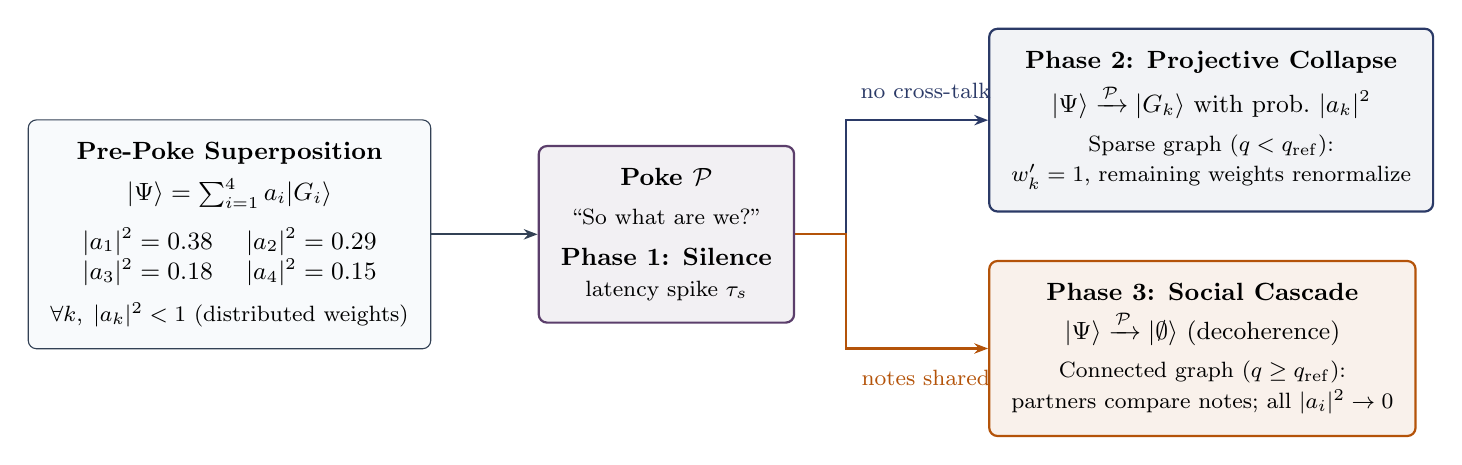
\begin{tikzpicture}[
  font=\small,
  box/.style={draw=slateink, rounded corners=3pt, fill=softbg, inner sep=8pt, align=center},
  pokebox/.style={draw=plumfill, thick, rounded corners=3pt, fill=plumfill!8, inner sep=8pt, align=center},
  outbox/.style={draw=navyfill, thick, rounded corners=3pt, fill=navyfill!6, inner sep=8pt, align=center},
  casbox/.style={draw=amberfill, thick, rounded corners=3pt, fill=amberfill!8, inner sep=8pt, align=center},
  arr/.style={-{Stealth[length=5pt]}, thick, slateink}
]

% Left: Pre-poke superposition
\node[box, minimum width=4.4cm] (pre) at (0, 0) {
  \textbf{Pre-Poke Superposition}\\[4pt]
  $\ket{\Psi} = \sum_{i=1}^{4} a_i \ket{G_i}$\\[6pt]
  \begin{tabular}{@{}ll@{}}
    $\lvert a_1\rvert^2 = 0.38$ & $\lvert a_2\rvert^2 = 0.29$\\
    $\lvert a_3\rvert^2 = 0.18$ & $\lvert a_4\rvert^2 = 0.15$
  \end{tabular}\\[4pt]
  {\footnotesize $\forall k,\; \lvert a_k\rvert^2 < 1$ (distributed weights)}
};

% Center: Poke operator
\node[pokebox, right=1.35cm of pre, minimum width=3.1cm] (poke) {
  \textbf{Poke $\mathcal{P}$}\\[3pt]
  {\footnotesize ``So what are we?''}\\[4pt]
  \textbf{Phase 1: Silence}\\
  {\footnotesize latency spike $\tau_s$}
};

% Right top: Projective collapse
\node[outbox, right=2.45cm of poke, yshift=1.45cm, minimum width=4.5cm] (proj) {
  \textbf{Phase 2: Projective Collapse}\\[3pt]
  $\ket{\Psi} \xrightarrow{\mathcal{P}} \ket{G_k}$ with prob.\ $\lvert a_k\rvert^2$\\[3pt]
  {\footnotesize Sparse graph ($q < q_{\mathrm{ref}}$):}\\
  {\footnotesize $w'_k = 1$, remaining weights renormalize}
};

% Right bottom: Cascade / decoherence
\node[casbox, right=2.45cm of poke, yshift=-1.45cm, minimum width=4.5cm] (cas) {
  \textbf{Phase 3: Social Cascade}\\[3pt]
  $\ket{\Psi} \xrightarrow{\mathcal{P}} \ket{\emptyset}$ (decoherence)\\[3pt]
  {\footnotesize Connected graph ($q \ge q_{\mathrm{ref}}$):}\\
  {\footnotesize partners compare notes; all $\lvert a_i\rvert^2 \to 0$}
};

\draw[arr] (pre.east) -- (poke.west);
\draw[arr, navyfill] (poke.east) -- ++(0.65, 0) |- (proj.west)
  node[pos=0.78, above=4pt, font=\footnotesize\color{navyfill}] {no cross-talk};
\draw[arr, amberfill] (poke.east) -- ++(0.65, 0) |- (cas.west)
  node[pos=0.78, below=4pt, font=\footnotesize\color{amberfill}] {notes shared};

\end{tikzpicture}
\end{document}
